\documentclass[12pt,a4paper]{scrartcl}
\usepackage[english]{babel}
\usepackage{url}
\usepackage{hyperref}

\hypersetup{
	colorlinks=true,
	urlcolor=black,
	linkcolor=black,
	citecolor=black
}
\usepackage{float}
\usepackage{graphicx}
\usepackage{listings}

\title{\large{Highly Available, Distributed and Fault Tolerant Storage System} \\ \normalsize{Distributed Systems 2011}}
\author{Karsten Westra\\1693905 \and Edwin-Jan Harmsma\\1735535}

\begin{document}
\maketitle

\tableofcontents
\clearpage


% @karsten: ik heb 'problem statement' en 'state of the art' omgewisseld
% omdat ik state of the art meer bij solution vind horen...

\section{Context}
% basics principles of storage systems
% key->value, distributed file systems, memcache
% introduce fault-tolerance (replication) and scalability

\section{Problem statement}
% introduce all requirements of our system
% show get, add, delete, set operations
% communication between different platforms
% show that basic idea is the same as file system (free list, file table, raw storage).

\section{State of the Art}
% introduce XOR idea (raid4 and raid5)
% asynchronous client-server, FIFO channels
% removing consistency issues --> less communication between instances 
% binary header-based protocol (platform independent)
% hash signing for security, client collects data by itself
% keeping connections open --> import for connection between storage services

\section{Solution details}
The layered architecture of the entire system is shown in \autoref{fig:layers}. There exist three layers, where the front-end layer below the client is optional. This layer is intended to make the client layer less complex and to improve some potential security issues, since it will hide all information about the actual underlying server infrastructure. With a front-end layer the client cannot trace the actual server instance that is storing a specific piece of a file or the actual server instance that stores the key of the file. Normally, this is not a very important issue, but it could make for example distributed denial-of-service attacks more easy.

The two arrows in \autoref{fig:layers} display the two different interfaces that are seen by the client. As mentioned above, if the front-end layer will be used the client will only use the use the public interface (GET, ADD, DELETE) that is indicated by \emph{arrow 1}. The front-end layer will forward this to the right dictionary server and collect the data from the storage service instances. \emph{Arrow 2} indicates the low level storage interface (READ, WRITE) that the client will use to respectively read or write the content of an entity. This interface might at first sight look a security vulnerability, but remember that the client can only use this interface with a valid timestamped signature that is granted by the dictionary service (by \emph{arrow 1}). So, this must ensure that it is impossible to write or read data randomly from a storage server, and this also explains why the front-end layer is optional.

\begin{figure}[H]
\centering
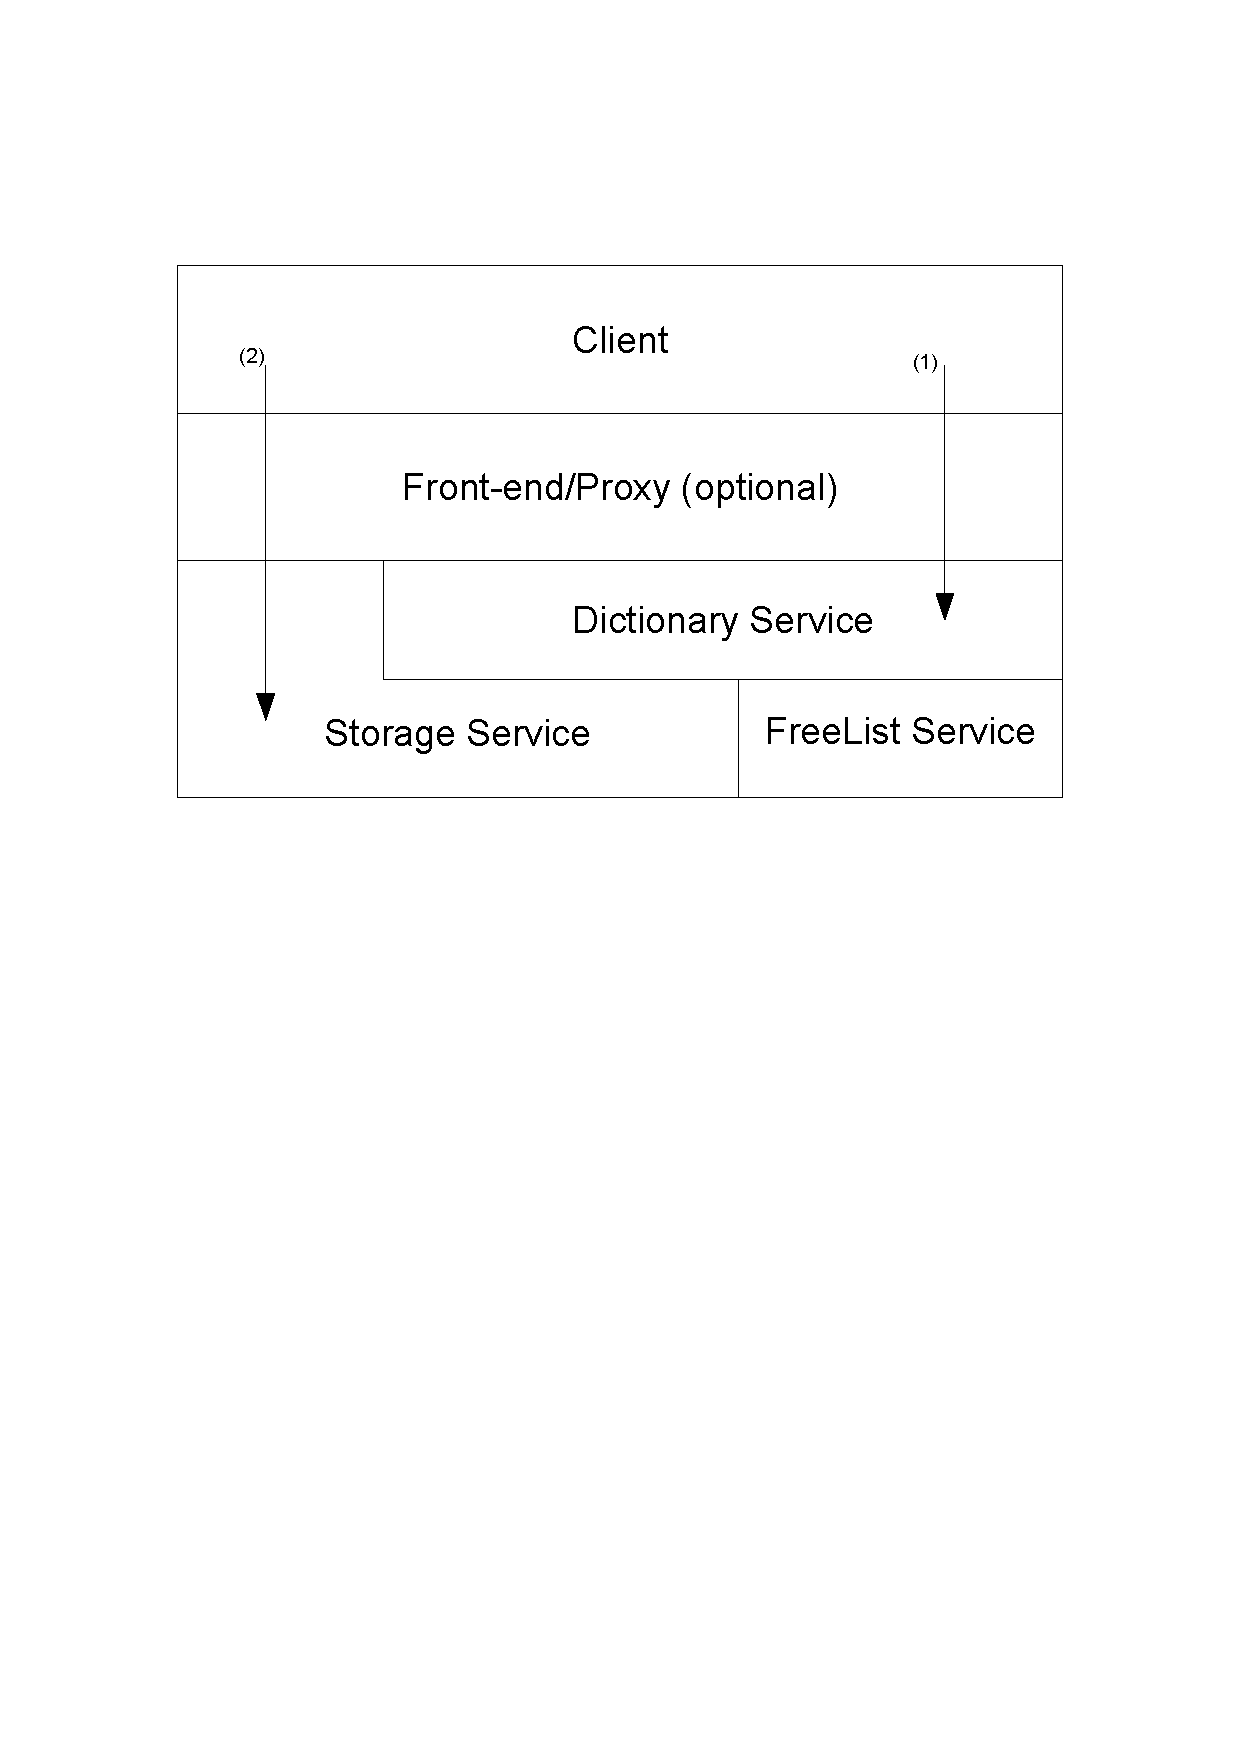
\includegraphics[width=0.8\textwidth,trim=1cm 16cm 1cm 4cm,clip=true]{diagrams/layer-architecture.pdf}
\caption{Layered architecture}
\label{fig:layers}
\end{figure}

In \autoref{fig:sequence-add} the sequence diagram of the ADD operation is shown. The ADD operation is shown because it is the most complex operation of all because it involves all other components. The front-end layer is not present in this diagram and the client will thus directly communicate with the Dictionary Services and Storage Services. Note that all objects in this diagram are distributed and require communication over a network. Also, the diagram suggests that for example \verb|write(offset, data)| completes in one step, but this is not the case in real life. Usually, these write actions are performed in multiple steps caused by of the buffering behavior of the underlying network  and the use of a network event library.

\begin{figure}[H]
\centering
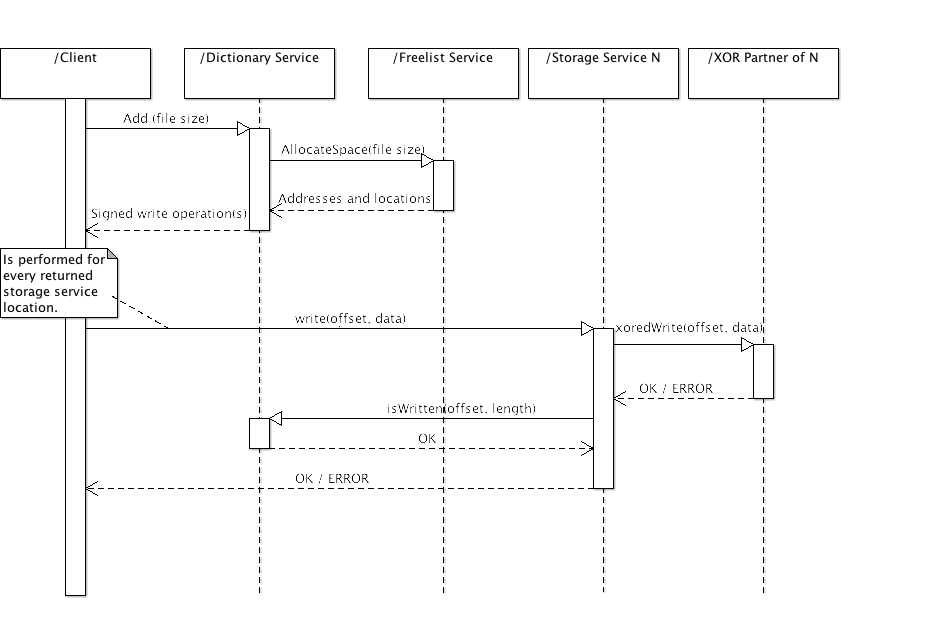
\includegraphics[width=\textwidth,trim=0 2cm 3cm 1cm,clip=true]{diagrams/add-operation.png}
\caption{Sequence diagram of the ADD operation. (Distributed communication within Dictionary Service and Freelist Service is not displayed for simplicity reasons.)}
\label{fig:sequence-add}
\end{figure}

The following subsections will discuss all the individual layers in more detail.


\subsection{Storage Service}
% talk about: write BEFORE read
% storagemanager... creation of RAID groups, standby servers
% chunked file writing: dataReceived() --> send to disk (could be zero copy)
% replication and XOR calculation...

\subsection{Dictionary Service}
\subsection{Freelist Service}
\subsection{Front-end / proxy}
\subsection{Client}
Without the optional front-end layer this layer must know the mapping from dictionary keys to dictionary server instance.

\section{Results}
% discuss also the properties that are explained in the DS lectures
% how fault-tollerant are we?

\section{Future improvements}
% system heavily relies on system clock (signing security) --> internal clock synchronization between components, is not implemented due the lack of time

% storage service:
% Remove blocking code between storageservice and parity server --> show blocking problem by sequence diagram, same for recovery
% Private key meganism, now every server has its own private key which is a big security issue --> only operation,offset,length/data are signed, NOT HOST/PORT!
% Reading from disk in chunks in order to prevent starvation of meerdere threads
% how errors must be handled: storage engine returns one error --> redo entire process, dictionary service will free unwritten entities

\bibliographystyle{plain}
\bibliography{ref}
\nocite{*}

\end{document}
